%!TEX root = Main.tex
\documentclass[Main]{subfiles}

\begin{document}

\section{Hardware} % (fold)
\label{sec:hardware}

	\subsection{Platform} % (fold)
	\label{sub:platform}

		The processing platform chosen for this project is a \emph{ZYBO Zynq™-7000 Development Board} from Digilent (see Figure \ref{fig:ZYBO}).
		The brains of the ZYBO is a Xilinx Zynq-7000 All Programmable System on a Chip (AP SoC).
		The AP SoC (see Figure \ref{fig:ZynqArch}) features both a Processing System (PS) consisting of 650 MHz dual core ARM\textregistered{} Cortex A9 CPU with dedicated I/O and Memory and extensible FPGA Programmable Logic (PL) for HW synthesis.

		This enables the construction of a system with software, written in C++, running on the CPU, and with dedicated hardware for acceleration of computation and I/O handling.
		\begin{figure}[H]
			\centering
			\begin{subfigure}[b]{0.55\linewidth}
				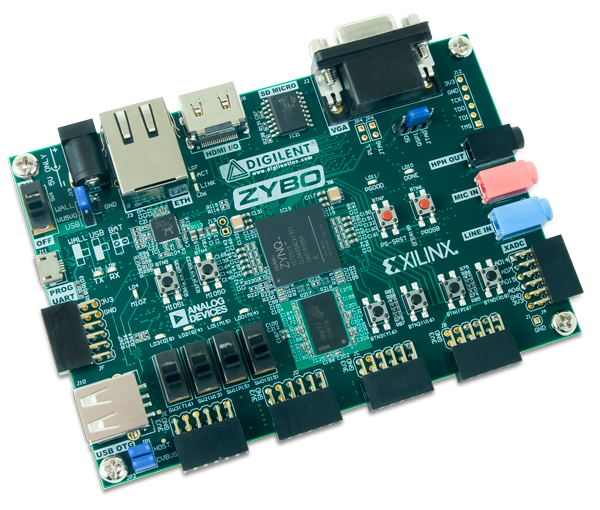
\includegraphics[width=\linewidth]{ZYBO}
				\caption{Digilent Zynq Board (ZYBO)}
				\label{fig:ZYBO}
			\end{subfigure}		
			\begin{subfigure}[b]{0.4\linewidth}
				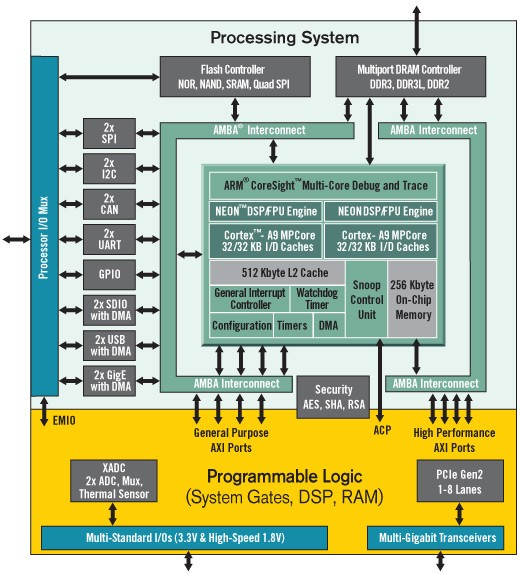
\includegraphics[width=\linewidth]{ZynqArch}
				\caption{Zynq-7000 AP SoC Diagram}
				\label{fig:ZynqArch}
			\end{subfigure}
			\caption{Figures borrowed from \cite{Digilent2014}}		
		\end{figure}

		Alongside the AP SoC the ZYBO features a range external hardware for power supply/management and interfacing.
		It has push-buttons, throw-switches and LEDs for direct interface, USB-OTG, UART-to-USB and Ethernet for communication and HDMI, VGA and an audio codec for Audio/Visual.

		Lastly, the ZYBO features six PMOD GPIO ports along the perimeter (see Figure \ref{fig:ZYBO}), one directly connected to the PS and the others accessible through the PL.
		They deliver 3.3V power to external devices as well as eight customizable 1.8V or 3.3V digital I/O ports each (see Figure \ref{fig:pmod}).
		These are used for interfacing with the sensor and motor (see Section \fxnote{ref to sensors} and \fxnote{ref to motors}, respectively).

		\begin{figure}[H]
			\centering
			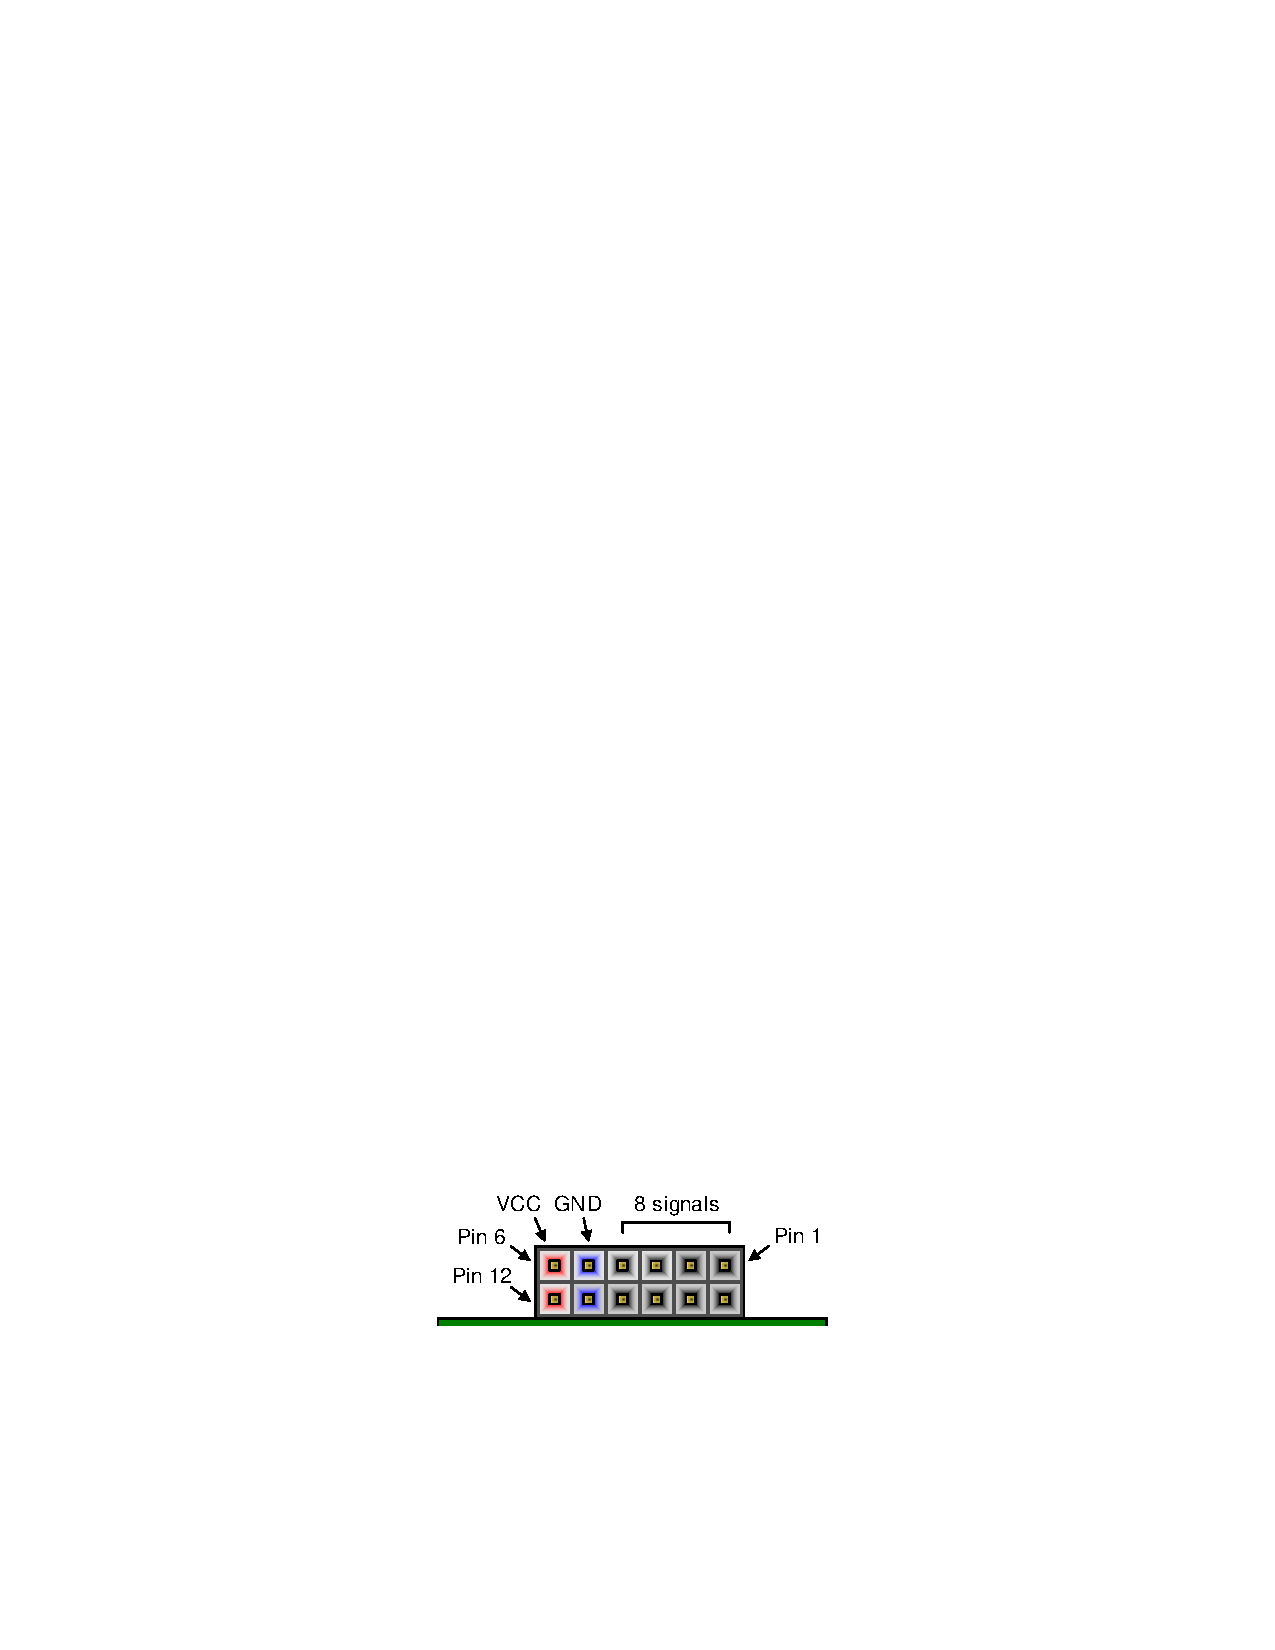
\includegraphics[width=0.5\linewidth]{PMOD_connector}
			\caption{PMOD Connector. Borrowed from \cite{Digilent2014}}
			\label{fig:pmod}
		\end{figure}


		\subsubsection{HW/SW Co-Design} % (fold)
		\label{ssub:hw_sw_co_design}

			The availability of FPGA logic on-chip enables rapid prototyping of HW acceleration blocks, through the use of High-Level Synthesis (HLS) tools.
			Using HLS one can specify some desired functionality in C++/SystemC code and directly synthesize it to HW-blocks to be implemented in FPGA logic, without needing to explicitly design HW in a Hardware Description Language like VHDL or Verilog.

			This is utilized for creating a PWM motor controller, described in Section \fxnote{ref to PWM controller HLS}.
			\fxnote{Section on Vidado desgin}

			% subsubsection hw_sw_co_design (end)
	
		% subsection platform (end)

	\subsection{Power} % (fold)
	\label{sub:power}
	
	% subsection power (end)

	\subsection{Sensors} % (fold)
	\label{sub:sensor}
	
	% subsection sensor (end)

	\subsection{Motor Control} % (fold)
	\label{sub:motor_control}

		The motor control hardware consists of two major blocks, an external Dual H-Bridge for driving the power the the motors, and an on-chip PWM controller for controlling the motor driver.
		The connection between the two blocks are shown in the SysML internal block diagram of the Motion block (\autoref{fig:motion_ibd}), along with the two motors.
		The \emph{Power}-signal comes from a battery, and \emph{Motor Control} is connected to the Processing System.

		\begin{figure}[H]
			\centering
			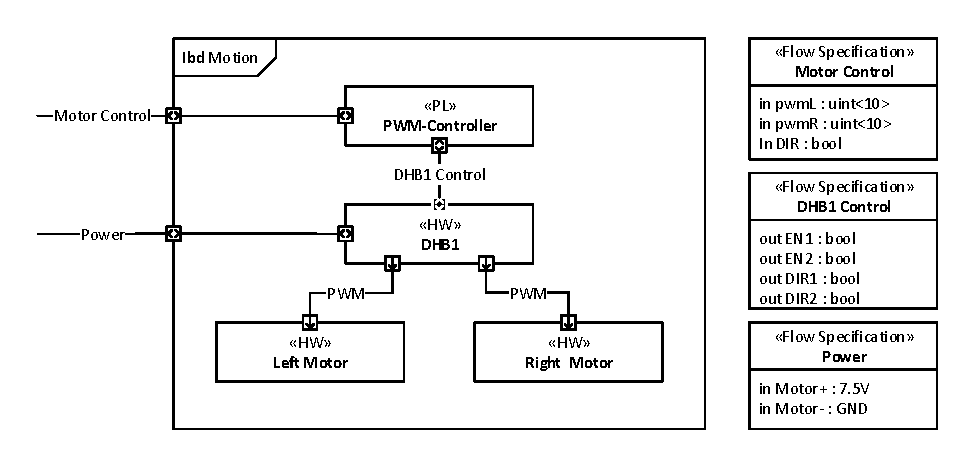
\includegraphics[width=1.0\linewidth]{MotionIBD}
			\caption{SysML Internal Block Diagram of the Motion Block}
			\label{fig:motion_ibd}
		\end{figure}


		\subsubsection{External Dual H-Bridge} % (fold)
		\label{ssub:external_dual_h_bridge}
			
			The \emph{DHB1} from Digilent is a dual- H-bridge motor controller that enables regular DC-motors to be driven in either direction with with a single ended power supply.
			Further it provides logic level transistor switching so that higher voltages (up to 11.8V) and higher currents (1.5A RMS, 2A peak) can be used to drive the motor without loading the logic circuit.

			\begin{figure}[H]
				\centering
				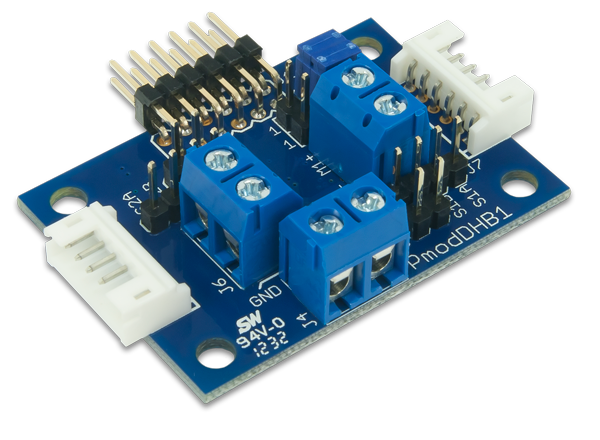
\includegraphics[width=0.5\linewidth]{PmodDHB1}
				\caption{Digilent PmodPHB1 Dual H-Bridge Motor controller \cite{Digilent2014}}
				\label{fig:DHB1}
			\end{figure}

			The DHB1 connects to the ZYBO via a PMOD connector. The individual signals signal are listed in \autoref{tab:dhb_pmod}.
			The motor power source is connected to the DHB1 with screw terminals. The two motors are also connected with screw terminals, but the left motor is connected reversed polarity.
			This is because the identical motors need to spin in different directions to achieve the same rotation in relation to the direction of travel.

			\begin{table}[H]
				\centering
				\begin{subtable}[b]{0.6\linewidth}
					\begin{tabular}{|c|l|l|}
						\hline
						{\bf Pin} & {\bf Signal} & {\bf Description}         \\ \hline
						1         & EN1          & Motor 1 Enable            \\ \hline
						2         & DIR1         & Motor 1 Direction         \\ \hline
						3         & S1A          & Motor 1 Sensor A Feedback \\ \hline
						4         & S1B          & Motor 1 Sensor B Feedback \\ \hline
						5         & GND          & Power Supply Ground       \\ \hline
						6         & $V_{CC}$     & Power Supply (3.3V)       \\ \hline
						7         & EN2          & Motor 2 Enable            \\ \hline
						8         & DIR2         & Motor 2 Direction         \\ \hline
						9         & S2A          & Motor 2 Sensor A Feedback \\ \hline
						10        & S2B          & Motor 2 Sensor B Feedback \\ \hline
						11        & GND          & Power Supply Ground       \\ \hline
						12        & $V_{CC}$   & Power Supply (3.3V)       \\ \hline
					\end{tabular}
					\caption{PMOD connection description}
					\label{tab:dhb_pmod}
				\end{subtable}
				\begin{subtable}[b]{0.3\linewidth}
					\centering
					\begin{tabular}{ccl}
						\hline
						\multicolumn{1}{|c|}{{\bf DIR1}} & \multicolumn{1}{c|}{{\bf EN1}} & \multicolumn{1}{l|}{{\bf Result M1}} \\ \hline
						\multicolumn{1}{|c|}{0}          & \multicolumn{1}{c|}{0}         & \multicolumn{1}{l|}{Stop}            \\ \hline
						\multicolumn{1}{|c|}{0}          & \multicolumn{1}{c|}{1/PWM}     & \multicolumn{1}{l|}{Forward}         \\ \hline
						\multicolumn{1}{|c|}{1}          & \multicolumn{1}{c|}{0}         & \multicolumn{1}{l|}{Stop}            \\ \hline
						\multicolumn{1}{|c|}{1}          & \multicolumn{1}{c|}{1/PWM}     & \multicolumn{1}{l|}{Reverse}         \\ \hline
						                                 &                                &                                      \\ \hline
						\multicolumn{1}{|c|}{{\bf DIR2}} & \multicolumn{1}{c|}{{\bf EN2}} & \multicolumn{1}{l|}{{\bf Result M2}} \\ \hline
						\multicolumn{1}{|c|}{0}          & \multicolumn{1}{c|}{0}         & \multicolumn{1}{l|}{Stop}            \\ \hline
						\multicolumn{1}{|c|}{0}          & \multicolumn{1}{c|}{1/PWM}     & \multicolumn{1}{l|}{Forward}         \\ \hline
						\multicolumn{1}{|c|}{1}          & \multicolumn{1}{c|}{0}         & \multicolumn{1}{l|}{Stop}            \\ \hline
						\multicolumn{1}{|c|}{1}          & \multicolumn{1}{c|}{1/PWM}     & \multicolumn{1}{l|}{Reverse}         \\ \hline
					\end{tabular}
					\caption{Truth table for DHB-1 input}
					\label{tab:motor_signal}
				\end{subtable}
				\caption{} 
			\end{table} 

			To control the direction of the motor one applies a logic level to the \emph{DIR} pin for the corresponding motor; 1 for forward, 0 for reverse.
			The speed of the motors are controlled by applying a Pulse Width Modulated (PWM) signal to the EN pin for the corresponding motor (see \autoref{tab:motor_signal}).
			The sensor feedback pins are not used as there are no sensors attached to the wheels.

			For more information, see the reference manual \cite{Digilent2014}.

			% subsubsection external_dual_h_bridge (end)

		\subsubsection{PWM-controller} % (fold)
		\label{ssub:pwm_controller}
			
			The PWM-controller is implemented in as a hardware IP-Core in the FPGA logic of the AP SoC.
			It has been modeled in SystemC code in the Vivado HLS tool.
			\autoref{lst:pwm_header} shows the header defining the PWM-controller module, consisting of a clock dividing thread and a PWM handling thread.
			It also defines the interface of \texttt{//Ports}, as designed in the IBD in \autoref{fig:motion_ibd}.

			\lstinputlisting[caption=PWM-Controller SystemC Header, style=Code-C++, label=lst:pwm_header, basicstyle=\scriptsize]{../MotorControl/MotorControl/main.h}

			\autoref{lst:pwm_definition} shows the definition of the module declared in \autoref{lst:pwm_header}.
			The \texttt{clockDividerThread} is responsible for dividing the 100 MHz clock of the PL down to a 2 MHz clock that can be used for ticks in the \texttt{pwmThread}.
			The use of a 2 MHz PWM-clock is based on the choice of a 10 bit resolution and a recommendation from \cite{Digilent2014} of a ~2 kHz PWM-cycle for the DHB1.

			\begin{equation}
				f_{PWMclock}
				\frac{f_{PL}}{ONE\_TICK} =
				\frac{100\ \text{MHz}}{25} =
				2\ \text{MHz}
			\end{equation}

			\begin{equation}
				f_{PWMcycle} =
				\frac{f_{PWMclock}}{2^{PWM\ resolution}} =
				\frac{2\ \text{MHz}}{2^{10}} =
				\frac{2\ \text{MHz}}{1024}} =
				1.953\ \text{kHz}
				\approx 2\ \text{kHz}
			\end{equation}

			\texttt{clockDividerThread} signals \texttt{pwmThread} of a PWM clock tick by setting \texttt{pwmClock} for one PL clock-cycle every time a PWM clock tick is generated.

			


			\lstinputlisting[caption=PWM-Controller SystemC Definition, style=Code-C++, label=lst:pwm_definition, basicstyle=\scriptsize]{../MotorControl/MotorControl/main.cpp}

			This model was then synthesized to VHDL code using the Vivado HLS tool and imported into the overall block design on 



			% subsubsection pwm_controller (end)
		
		% subsection motor_control (end)

	% section hardware (end)

\end{document}